\documentclass{article}

\usepackage{tikz}
\usetikzlibrary{calc}
\usepackage{xcolor}
\usepackage{graphicx}

\usepackage[
  paperwidth=35.5cm,
  paperheight=23cm,
  margin=0cm
]{geometry}

\pagestyle{empty}

\begin{document}

\begin{tikzpicture}[remember picture,overlay]

% =========================
% FUNDO
% =========================
\shade[top color=gray!10,bottom color=black!40]
(current page.south west) rectangle (current page.north east);

% =========================
% DIMENSÕES
% =========================
\pgfmathsetmacro{\pagewidth}{35.5}
\pgfmathsetmacro{\pageheight}{23}
\pgfmathsetmacro{\spinewidth}{1.3}

\pgfmathsetmacro{\halfwidth}{\pagewidth/2}
\pgfmathsetmacro{\side}{(\pagewidth - \spinewidth)/2}

% =========================
% PONTOS BASE
% =========================
\coordinate (center) at (current page.center);
\coordinate (front) at ($(center)+(\side/2,0)$);
\coordinate (back)  at ($(center)-(\side/2,0)$);

% =========================
% CAPA (DIREITA)
% =========================

\node[align=center, text=black]
at ($(front)+(0,5)$)
{
{\Huge\bfseries Processamento Digital de Imagens}\\[0.6cm]
{\large Uma abordagem interativa com {\ttfamily p5.js}}
};

\node[align=center, text=black]
at ($(front)+(0,-5)$)
{\large Luiz Eduardo da Silva};

% =========================
% CONTRACAPA (ESQUERDA)
% =========================

\node[text=black!80, align=center]
at ($(center)+(-8,0)$)
{
\small
Este livro apresenta conceitos fundamentais de\\
Processamento Digital de Imagens com abordagem\\
visual e interativa.\\[0.5cm]

Inclui exemplos práticos utilizando {\ttfamily p5.js}.
};

\node[text=black!80]
at ($(center)+(-8,-6)$)
{\small 2026};

% =========================
% LOMBADA
% =========================

\node[rotate=90, text=black]
at (center)
{\large Processamento Digital de Imagens};

% =========================
% IMAGENS
% =========================
\begin{scope}[opacity=0.15]

\node at ($(center)+(10,6)$)
{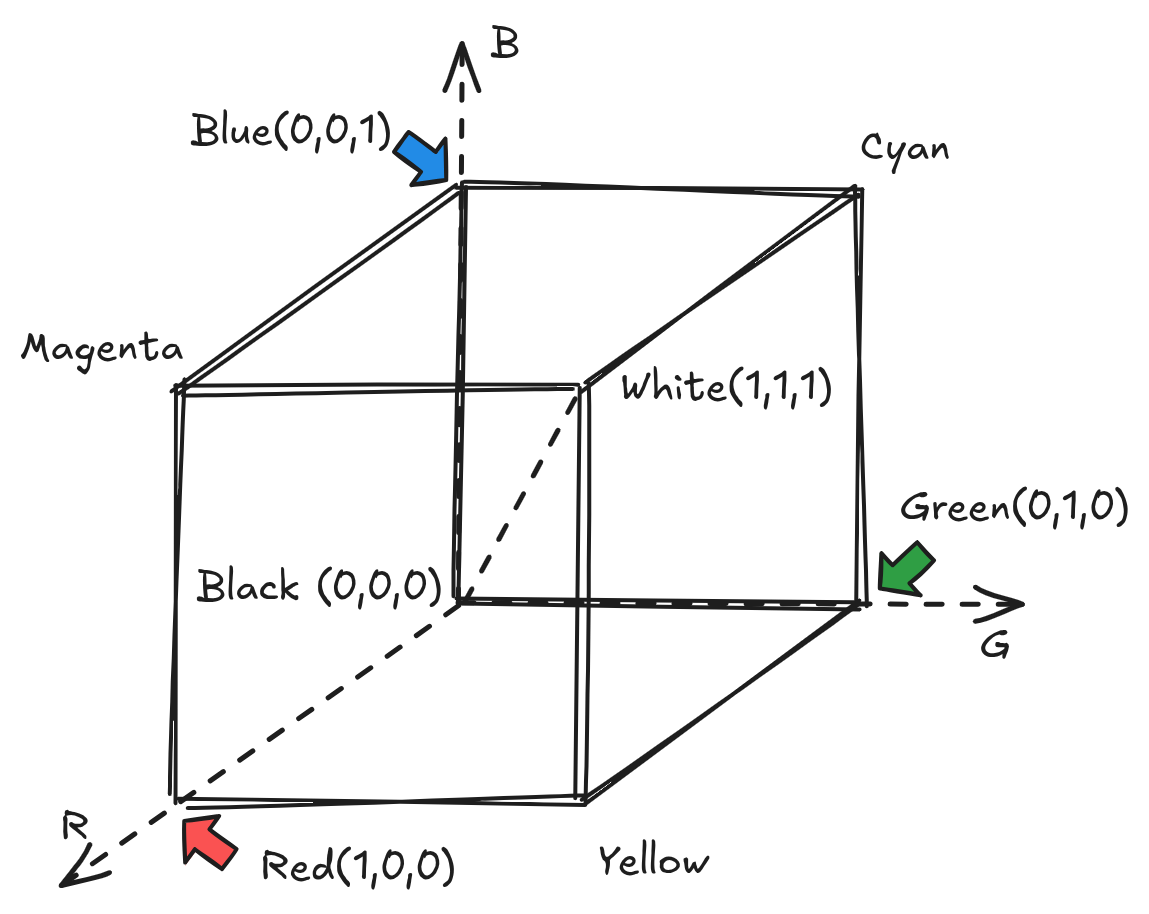
\includegraphics[width=8cm]{rgb.png}};

\node at ($(center)+(-10,6)$)
{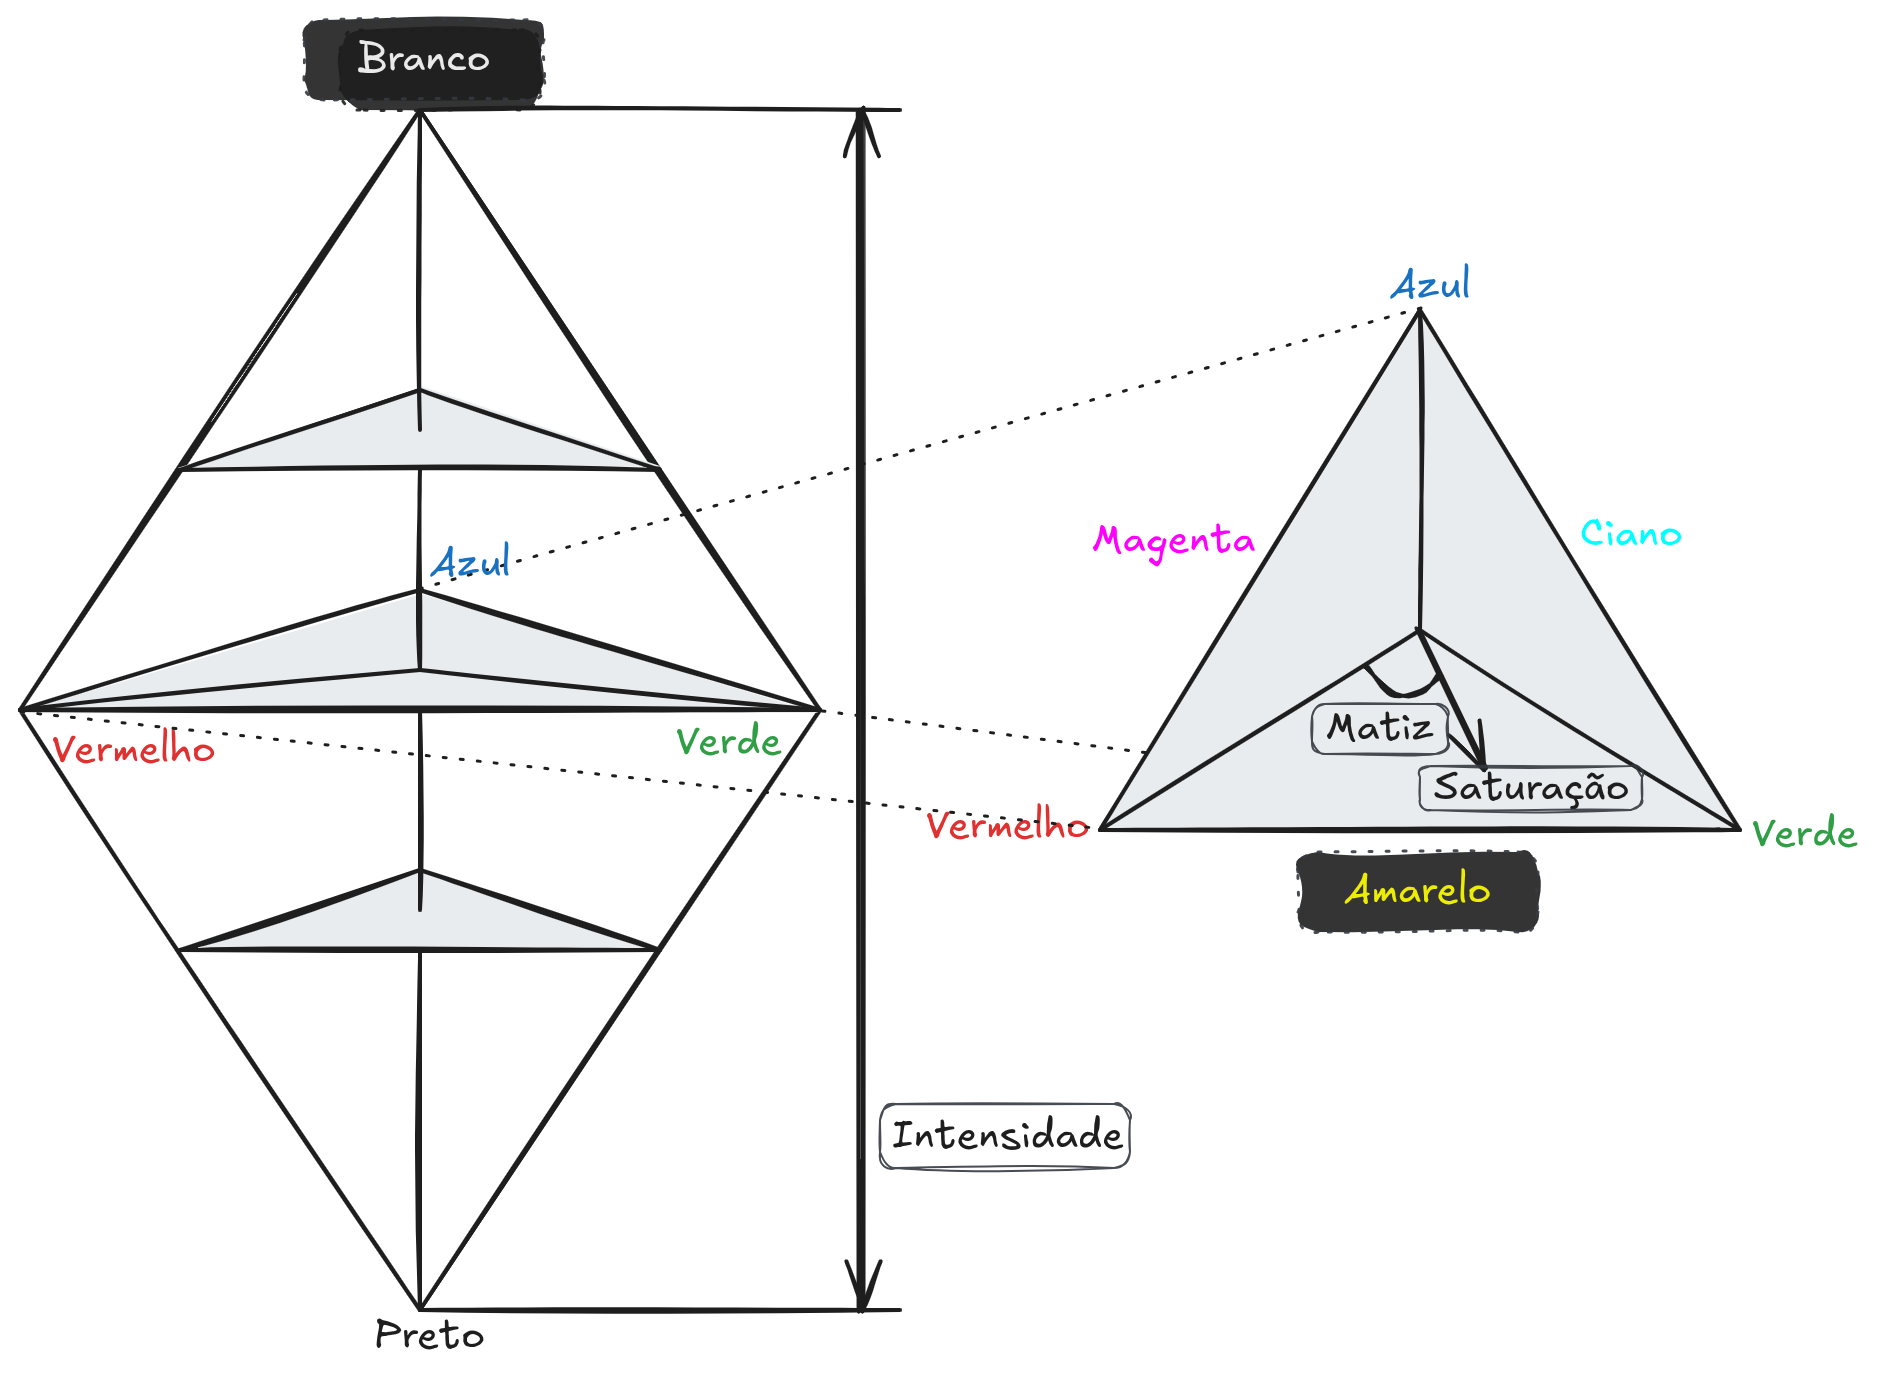
\includegraphics[width=8cm]{hsi.png}};

\node at ($(center)+(10,-6)$)
{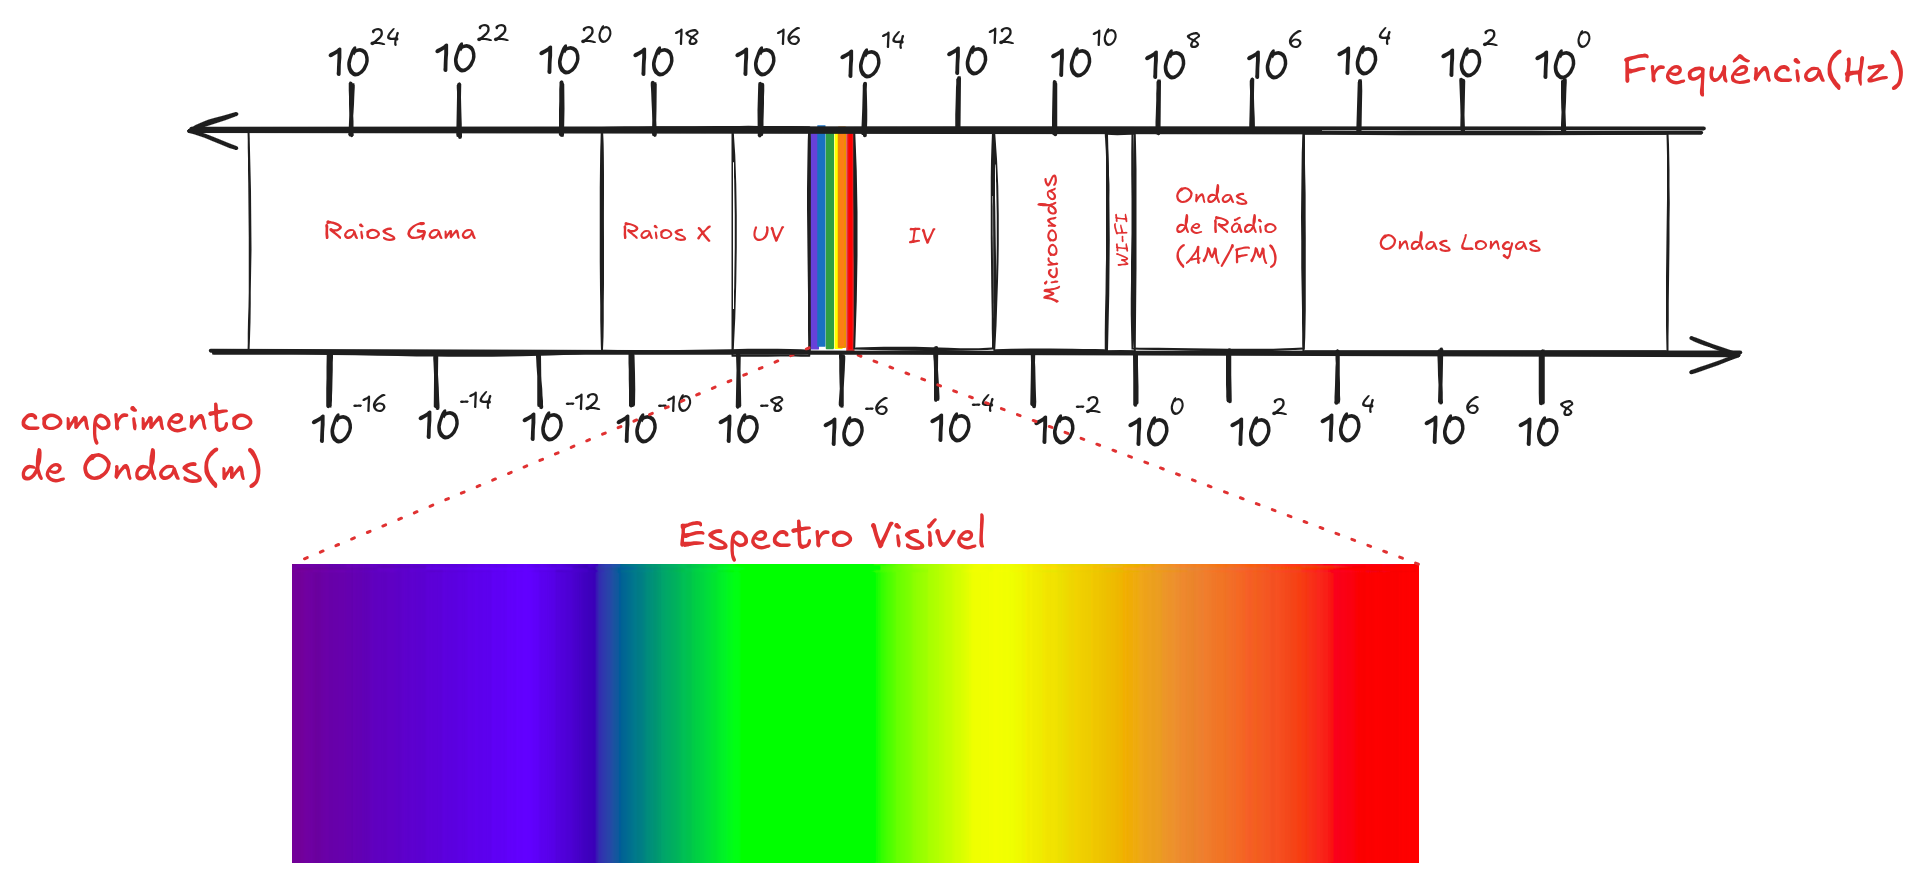
\includegraphics[width=10cm]{espectro.png}};

\node at ($(center)+(-10,-4)$)
{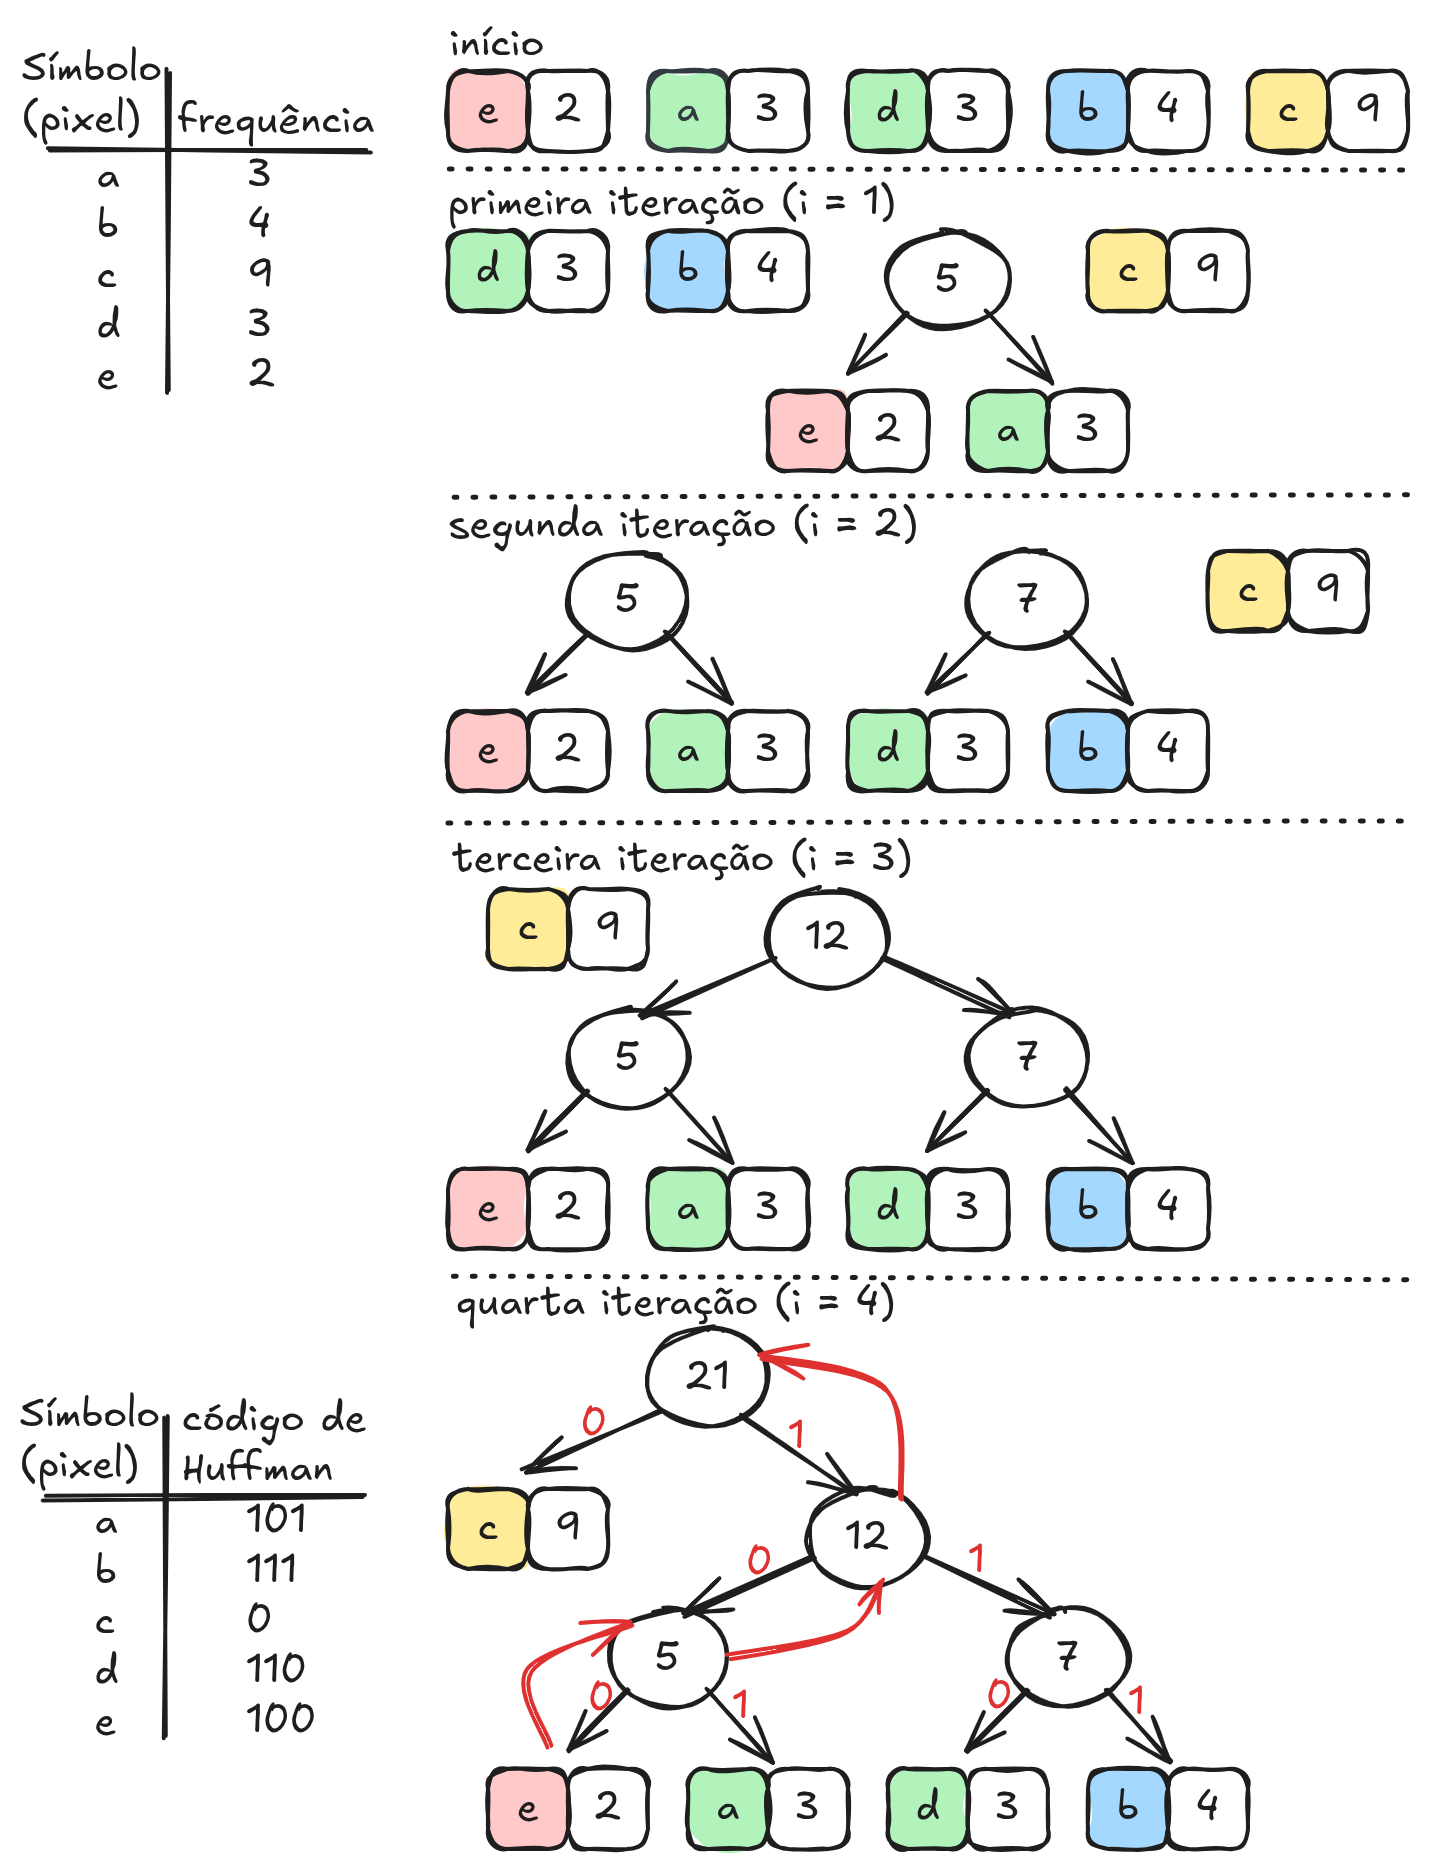
\includegraphics[width=8cm]{huffman.png}};

\node at ($(center)+(0,-6)$)
{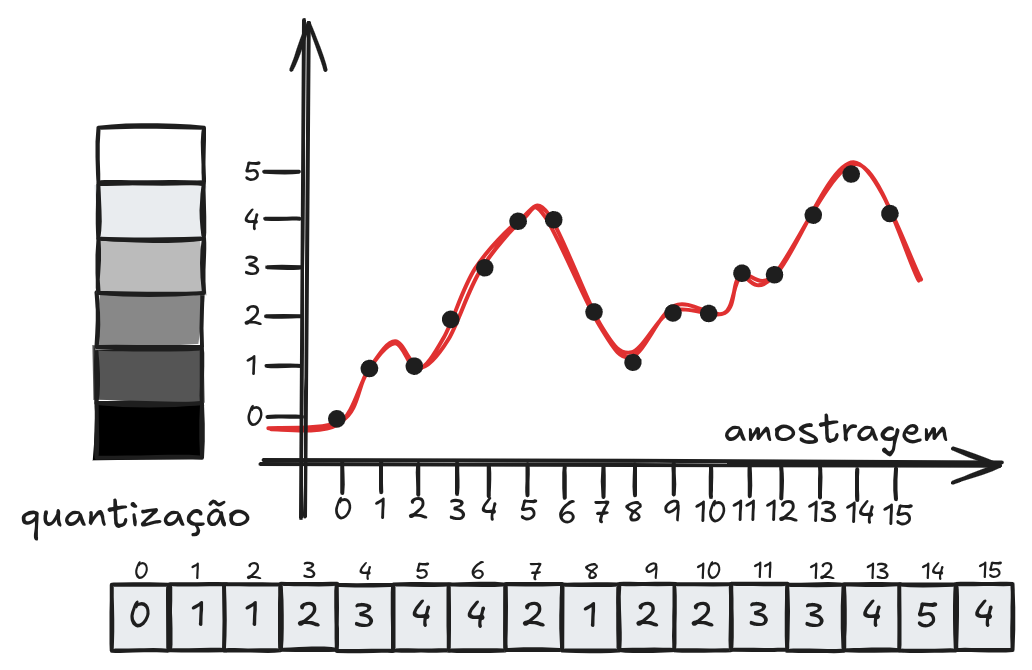
\includegraphics[width=6cm]{amostragem.png}};

\node at ($(center)+(10,0)$)
{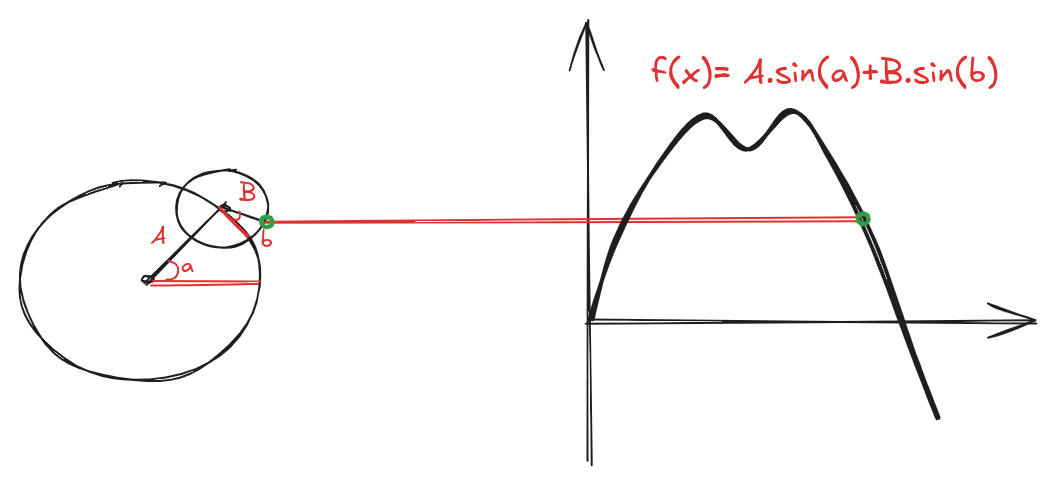
\includegraphics[width=10cm]{epiciclo.png}};

\node at ($(center)+(0,6)$)
{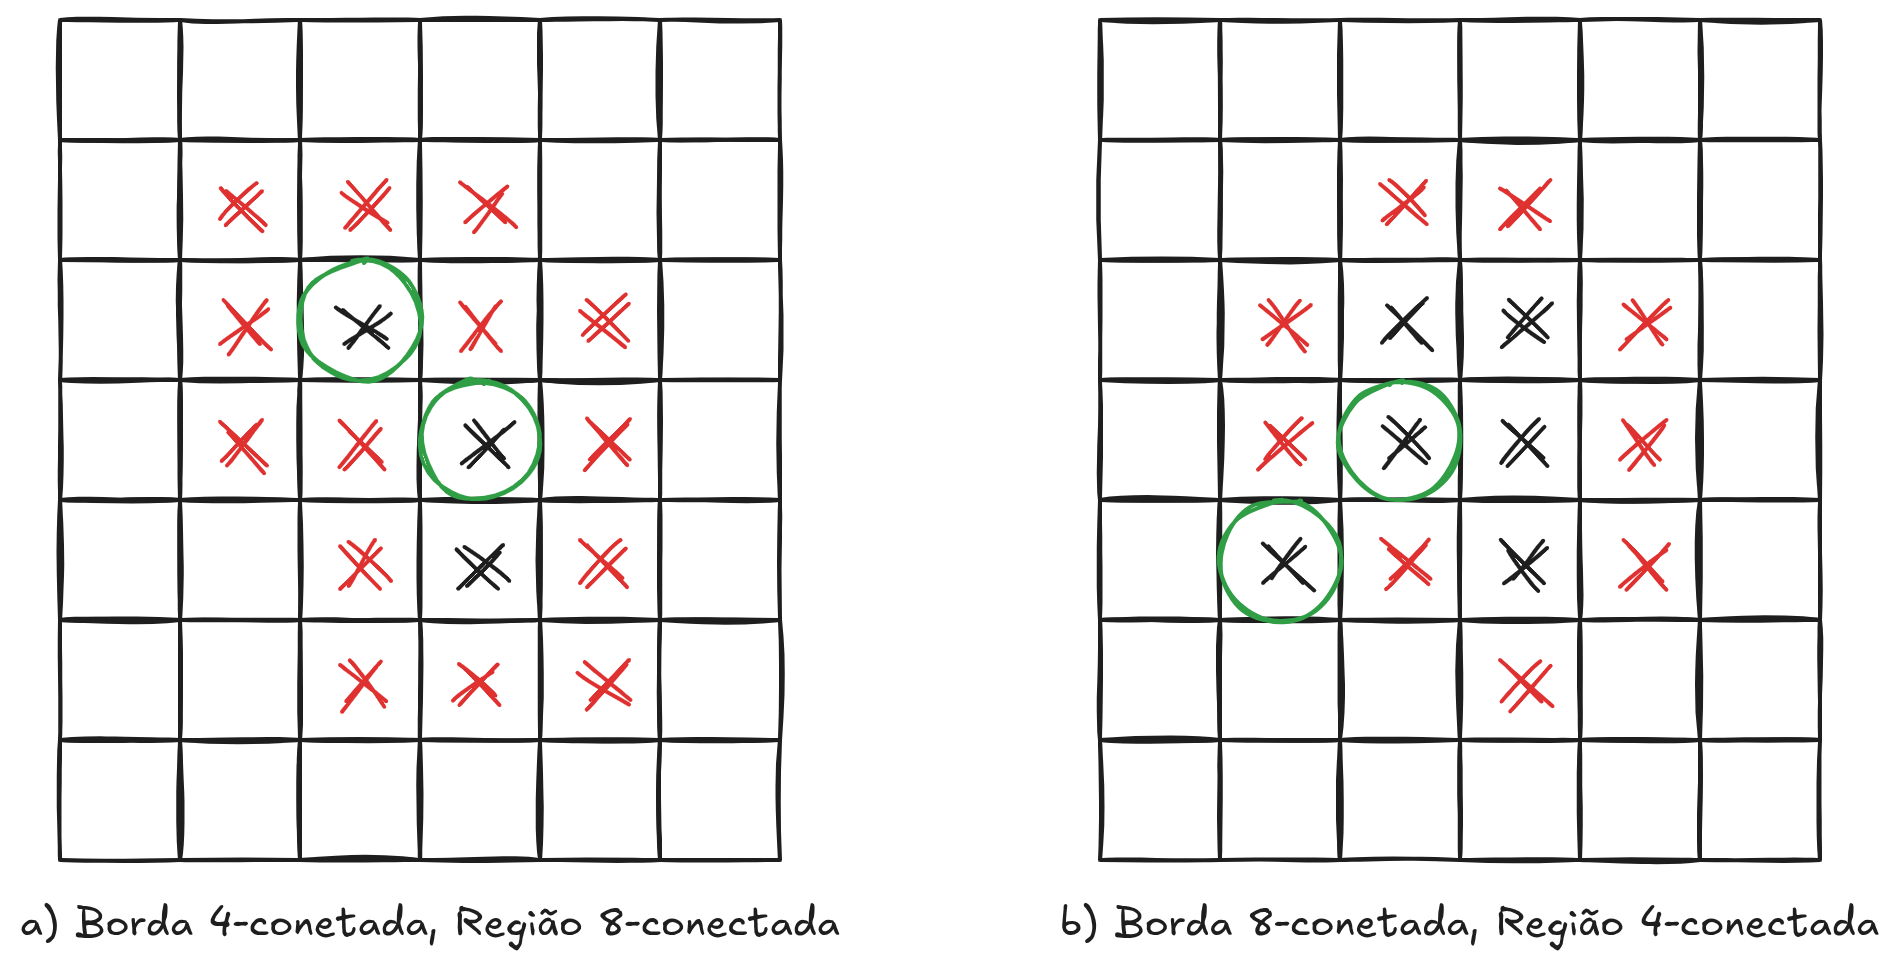
\includegraphics[width=6cm]{paradoxo.png}};

\end{scope}

\end{tikzpicture}

\end{document}